\documentclass[preview]{standalone}

\usepackage{amsmath}
\usepackage{amssymb}
\usepackage{stellar}
\usepackage{definitions}
\usepackage{bettelini}
\usepackage{tikz}
\usetikzlibrary{arrows.meta}

\begin{document}

\id{surface-orientation}
\genpage

\section{Surface Orientation}

\begin{snippet}{top-exterior-power-orientation-interpretation}
    If \(V\) is a \(k\)-dimensional real vector space, its top exterior
    power \(\bigwedge^kV^*\) is one-dimensional. Choosing either connected
    component of its nonzero elements determines an orientation of \(V\).
    An orientation of a surface requires these choices to vary coherently
    from one tangent space to the next.
\end{snippet}

\begin{snippetdefinition}{orientable-surface-definition}{Orientable surface}
    A regular surface \(\Sigma\subseteq\realnumbers^3\) is
    \emph{orientable} if it admits a continuous unit normal field
    \[
        \nu\colon\Sigma\fromto\realnumbers^3.
    \]
    An \emph{orientation} is a choice of one of the two such normal
    directions. More generally, a \(k\)-dimensional manifold is orientable
    when its tangent spaces admit a coherent orientation.
\end{snippetdefinition}

\begin{snippet}{nonorientable-surface-examples}
    The Möbius strip is a surface with boundary that is not orientable. The
    Klein bottle is a nonorientable surface without boundary; it cannot be
    embedded in \(\realnumbers^3\) without self-intersections.
\end{snippet}

\begin{snippetexample}{mobius-strip-nonorientability-example}{Möbius strip}
    A Möbius strip can be parametrized by
    \[
        \sigma(u,v)=
        \left(
            \left(1+\frac v2\cos\frac u2\right)\cos u,
            \left(1+\frac v2\cos\frac u2\right)\sin u,
            \frac v2\sin\frac u2
        \right),
    \]
    with \(u\in[0,2\pi]\) and \(v\in[-1,1]\). The parameter \(u\)
    rotates the strip around the \(z\)-axis, while \(v\) runs along each
    transverse segment. During one full revolution, that segment performs a
    half-turn.

    \begin{center}
        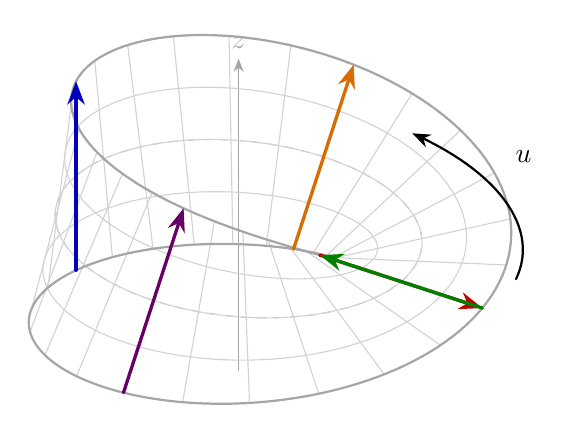
\begin{tikzpicture}[
                scale=2.4,
                x={(0.86cm,-0.28cm)},
                y={(0.45cm,0.38cm)},
                z={(0cm,1cm)},
                line cap=round,
                line join=round,
                >=Stealth
            ]

            \draw[->, gray!70] (0,0,-0.75) -- (0,0,0.9) node[above] {$z$};

            \draw[dashed, gray!55]
            plot[domain=0:360, samples=120, variable=\ang]
            ({cos(\ang)}, {sin(\ang)}, {0});

            \foreach \seg in {-1,-0.5,0,0.5,1} {
                \draw[gray!35, thin]
                plot[domain=0:360, samples=120, variable=\ang]
                ({(1 + 0.5*\seg*cos(\ang/2))*cos(\ang)},
                    {(1 + 0.5*\seg*cos(\ang/2))*sin(\ang)},
                {0.5*\seg*sin(\ang/2)});
            }

            \foreach \ang in {0,15,...,360} {
                \draw[gray!35, thin]
                ({(1 + 0.5*(-1)*cos(\ang/2))*cos(\ang)},
                    {(1 + 0.5*(-1)*cos(\ang/2))*sin(\ang)},
                {0.5*(-1)*sin(\ang/2)})
                --
                ({(1 + 0.5*(1)*cos(\ang/2))*cos(\ang)},
                    {(1 + 0.5*(1)*cos(\ang/2))*sin(\ang)},
                {0.5*(1)*sin(\ang/2)});
            }

            \foreach \seg in {-1,1} {
                \draw[thick, gray!70]
                plot[domain=0:360, samples=160, variable=\ang]
                ({(1 + 0.5*\seg*cos(\ang/2))*cos(\ang)},
                    {(1 + 0.5*\seg*cos(\ang/2))*sin(\ang)},
                {0.5*\seg*sin(\ang/2)});
            }

            \foreach \ang/\col/\lab in {
                0/red!75!black/{$u=0$},
                90/orange!85!black/{$u=\frac{\pi}{2}$},
                180/blue!75!black/{$u=\pi$},
                270/violet!80!black/{$u=\frac{3\pi}{2}$},
                360/green!50!black/{$u=2\pi$}
            } {
                \draw[very thick, \col, ->]
                ({(1 + 0.5*(-1)*cos(\ang/2))*cos(\ang)},
                    {(1 + 0.5*(-1)*cos(\ang/2))*sin(\ang)},
                {0.5*(-1)*sin(\ang/2)})
                --
                ({(1 + 0.5*(1)*cos(\ang/2))*cos(\ang)},
                    {(1 + 0.5*(1)*cos(\ang/2))*sin(\ang)},
                {0.5*(1)*sin(\ang/2)});

                %\node[\col, font=\scriptsize] at
                %    ({1.35*cos(\ang)}, {1.35*sin(\ang)}, {0.25})
                %    {\lab};
            }

            \draw[->, thick]
            plot[domain=15:80, samples=30, variable=\ang]
            ({1.55*cos(\ang)}, {1.55*sin(\ang)}, {0});

            \node at ({1.75*cos(55)}, {1.75*sin(55)}, {0.12}) {$u$};

        \end{tikzpicture}
    \end{center}

    A normal transported continuously around the central circle returns
    with the opposite sign. Hence no globally continuous choice of unit
    normal exists, so the strip is nonorientable.
\end{snippetexample}

\section{Exercise}

\begin{snippetexercise}{sphere-surface-integral-radius-optimization-exercise}{Optimizing a surface integral over spheres}
    For \(R>0\), let
    \[
        f(R)=\iint_{S_R}
        \frac{|x|-z^2}{\sqrt{x^2+y^2+z^2}}\,dS,
    \]
    where \(S_R\) is the sphere of radius \(R\) centered at the origin.
    Determine the value of \(R\) that maximizes \(f(R)\).
\end{snippetexercise}

\begin{snippetsolution}{sphere-surface-integral-radius-optimization-solution}{Optimizing a surface integral over spheres}
    Use spherical coordinates
    \[
        \sigma(\varphi,\theta)=
        (R\sin\varphi\cos\theta,
         R\sin\varphi\sin\theta,
         R\cos\varphi),
    \]
    with \(dS=R^2\sin\varphi\,d\varphi\,d\theta\). Then
    \begin{align*}
        f(R)
        &=R^2\integral[0][2\pi]
        [\integral[0][\pi]
        [(|\sin\varphi\cos\theta|-R\cos^2\varphi)\sin\varphi]
        [\varphi]][\theta]\\
        &=R^2\left(
            \integral[0][2\pi][|\cos\theta|][\theta]
            \integral[0][\pi][\sin^2\varphi][\varphi]
            -2\pi R\integral[0][\pi]
            [\sin\varphi\cos^2\varphi][\varphi]
        \right)\\
        &=2\pi R^2-\frac{4\pi}{3}R^3.
    \end{align*}
    Here
    \[
        \int_0^{2\pi}|\cos\theta|\,d\theta=4,
        \qquad
        \int_0^\pi\sin^2\varphi\,d\varphi=\frac\pi2,
        \qquad
        \int_0^\pi\sin\varphi\cos^2\varphi\,d\varphi=\frac23.
    \]
    Thus \(f'(R)=4\pi R(1-R)\). On \((0,+\infty)\), the maximum is
    attained at \(R=1\), with \(f(1)=2\pi/3\).
\end{snippetsolution}

\end{document}
